\section{Design}
\subsection{Service Integrations}

irpSSHa is designed to be as simple as possible, while still providing users the ability to query large datasets, i.e., flow logs containing thousands or millions of records, efficiently, as well as the option to store the logs and query results securely in the cloud for future reference. This is achieved by integrating with the services Amazon Simple Secure Storage (S3) and Amazon Athena, both products offered by Amazon Web Services (AWS). S3 stores objects consisting of files and metadata in online storage containers called buckets that offer fine-grained access control rules. Athena is a service that allows running standard SQL queries against formatted data stored in S3; Athena is serverless and scales automatically to ensure ad-hoc queries remain performant regardless of dataset size. Integrating with these services means that users of irpSSHa must be able to provide valid AWS credentials for an account with access to both S3 and Athena. This restriction is acknowledged as a tradeoff for the performance, reliability, and ease of querying and storing large amounts of data that the services bring to irpSSHa. Future work could involve exploring ways to evolve irpSSHa to have fewer or no third party dependencies.

As necessitated by the automatic abusive IP reporting functionality in irpSSHa, the tool also integrates with the AbuseIPDB API. In addition to reporting IPs, irpSSHa queries AbuseIPDB for data on file about IPs identified as potential attackers from the input data in order to corroborate suspicions that a given IP is engaging in an SSH brute force attack. Using a free account with AbuseIPDB incurs a rate limit of 1000 requests per day, so future extended work would require an account tier upgrade.

\subsection{Input Requirements}

IP flow logs are required as input to irpSSHa in order to report on attackers. Because SSH uses TCP, logs containing only TCP flows would be sufficient. In an effort to simplify the tool, rather than reading streams of data at the packet resolution, irpSSHa requires packets to be aggregated into flows prior to running the analysis. Output generated from existing tools like NetFlow and AWS VPC Flow Logs can be used as input, or individual packet traffic could be preprocessed before running irpSSHa. The format of the input must match the expected format of the tool in order to run ad-hoc SQL queries as needed. The default format is modeled after the output from VPC Flow Logs and can be seen in Figure~\ref{fig:input-format}. Sample input adhering to this format can be seen in Figure~\ref{fig:sample-input}. The current format may appear a bit verbose; however, changing the format to match flow input data from different sources requires only a trivial change to the \texttt{create\_table} method in \texttt{athena\_helper.py}. More sample input files can be found in the irpSSHa GitHub repository. 


\subsection{Detailed Implementation}

irpSSHa is written in Python and relies on the AWS SDK for Python---\texttt{boto3}---and the \texttt{requests} Python module for its service integrations. 

Execution begins by uploading the input file to S3. This involves creating a bucket for the irpSSHa data if it does not exist yet, and uploading the input to a new uniquely named folder. Next, a database is created in Athena if one for irpSSHa does not exist, and then a table is created in the database with the default or modified field format. This table is configured by irpSSHa to automatically import the data from the appropriate bucket and folder in S3. At this point, the flow logs can be queried with standard SQL. irpSSHa executes the query in Figure~\ref{fig:query} to obtain a list of potential threats.

Once these IPs are identified by the query, irpSSHa issues a GET request to the AbuseIPDB API for each one and parses the response to record the number of times it has been reported for abusive activity in the past 60 days, as well as the number of those reports that implicated the IP in attacks with the "SSH" or "Brute Force" label, or both. 

\vspace{6em}

\begin{figure}[h]
%\resizebox{\textwidth}{!}
{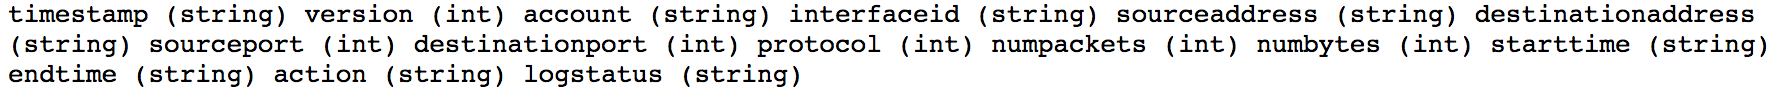
\includegraphics[width=3.5in]{./figures/561-default-format.png}}
%{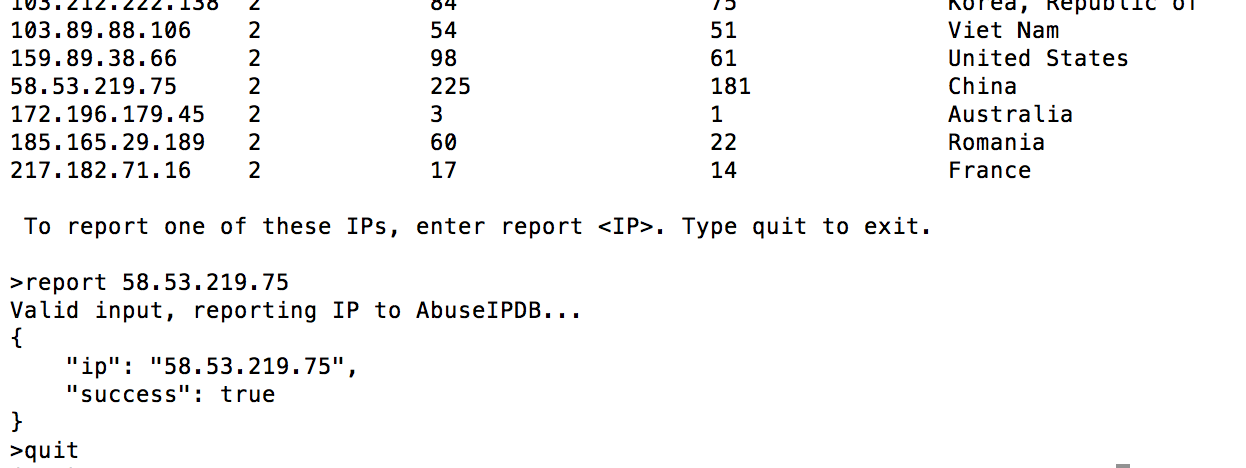
\includegraphics{./figures/561-irpSSHa-prompt.png}}
\caption{\small{Default input format}}
\label{fig:input-format}
\end{figure}

\begin{figure}[h]
%\resizebox{\textwidth}{!}
{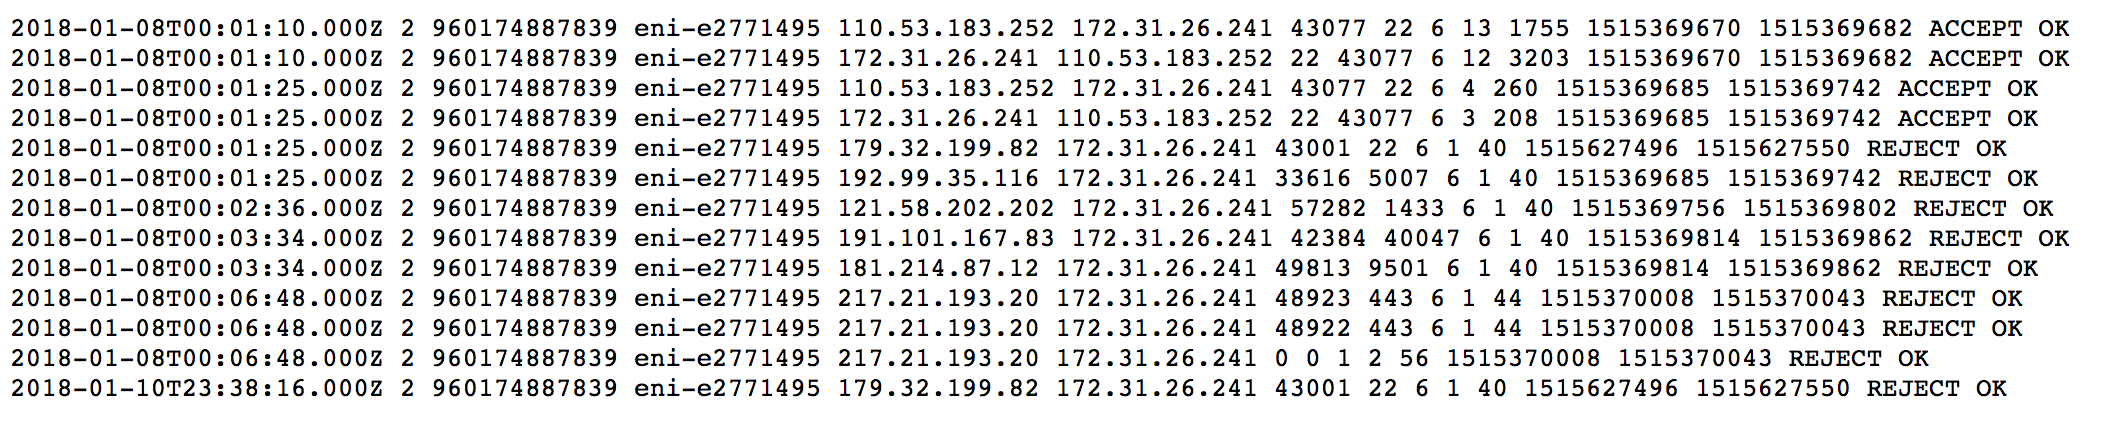
\includegraphics[width=4in]{./figures/561-sample-input.png}}
%{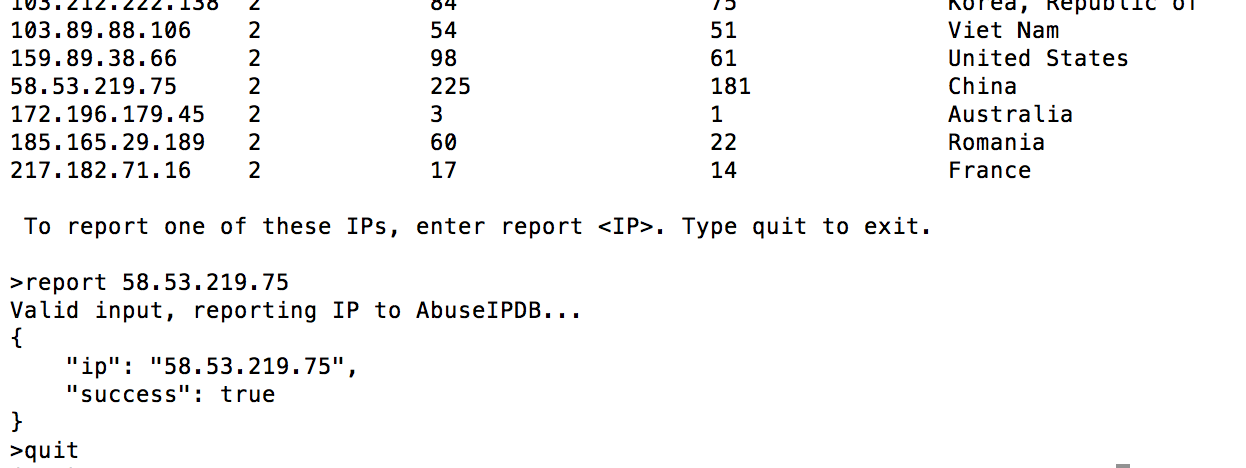
\includegraphics{./figures/561-irpSSHa-prompt.png}}
\caption{\small{Example of valid input in default format}}
\label{fig:sample-input}
\end{figure}

\begin{figure}[H]
%\resizebox{\textwidth}{!}
{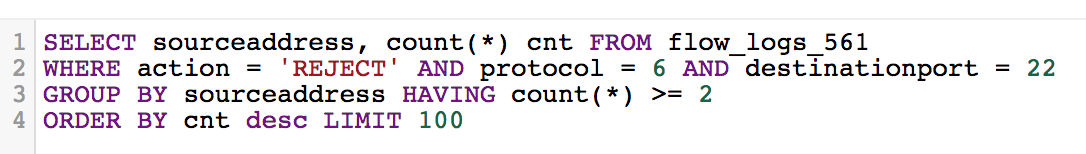
\includegraphics[width=3in]{./figures/561-athena-query.png}}
%{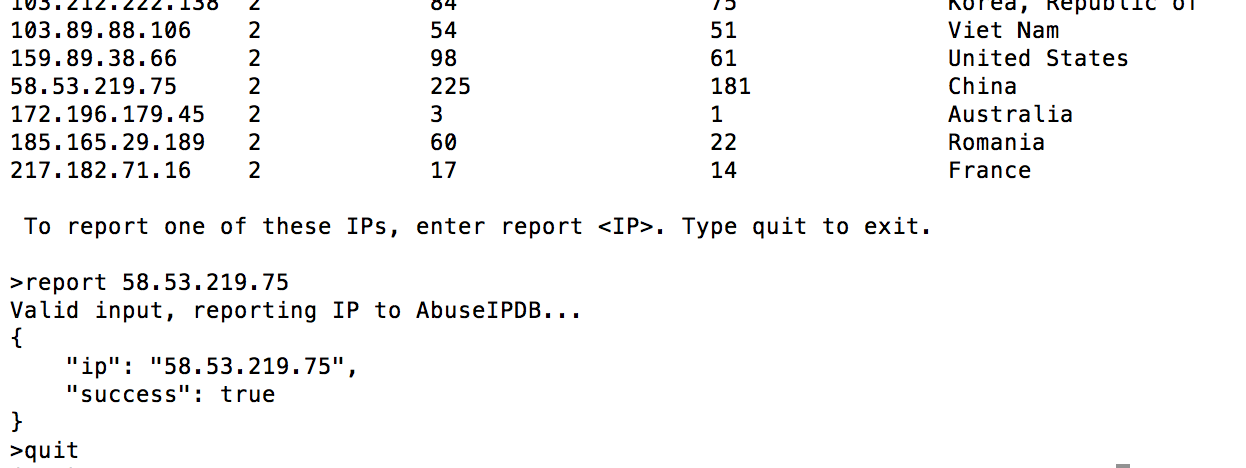
\includegraphics{./figures/561-irpSSHa-prompt.png}}
\caption{\small{Default SQL query used to identify potential attackers}}
\label{fig:query}
\end{figure}

After this information is obtained from the API for all IPs returned by the Athena query, the findings are presented to the user, along with an interactive prompt on the command line as shown in Figure~\ref{fig:prompt}. The user then has the option to review the results and select which, if any, of the source IPs to report. Entering \texttt{report <source IP>} with one of the IPs from the output will submit a report to AbuseIPDB via an HTTP POST. The report is submitted with the default or custom comment and is automatically tagged with categories "SSH" and "Brute Force". The report is then immediately viewable on the AbuseIPDB site, as shown in Figure~\ref{fig:report}.

\subsection{Additional Requirements}

It is recommended that the destination hosts for the input flows be secured enough to reject
unauthorized SSH traffic. In particular, ssh login should require public-key authentication and only whitelisted IPs should be allowed on the port running SSH, as discussed in Section 1.

\begin{figure}[H]
%\resizebox{\textwidth}{!}
{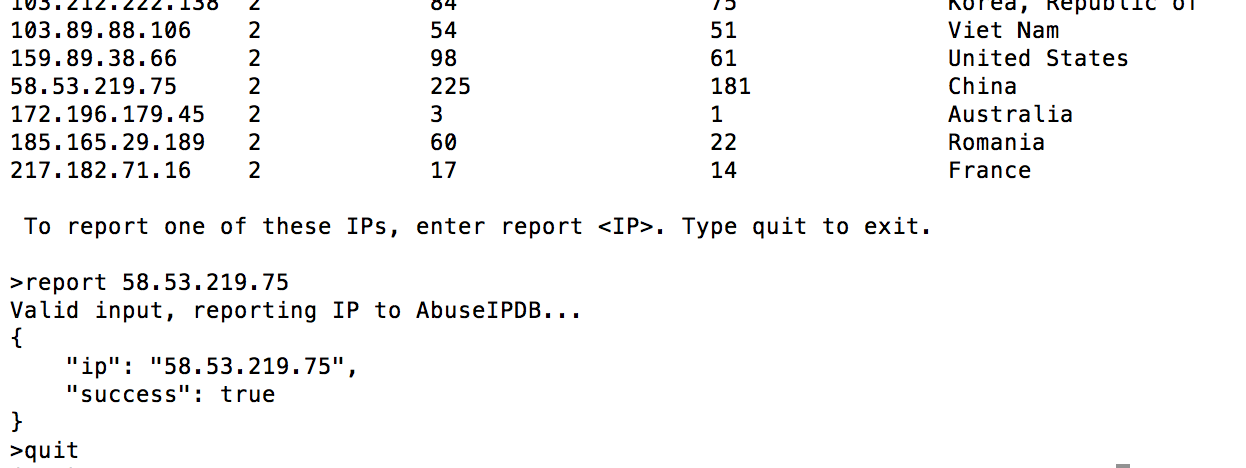
\includegraphics[width=3in]{./figures/561-irpSSHa-prompt.png}}
%{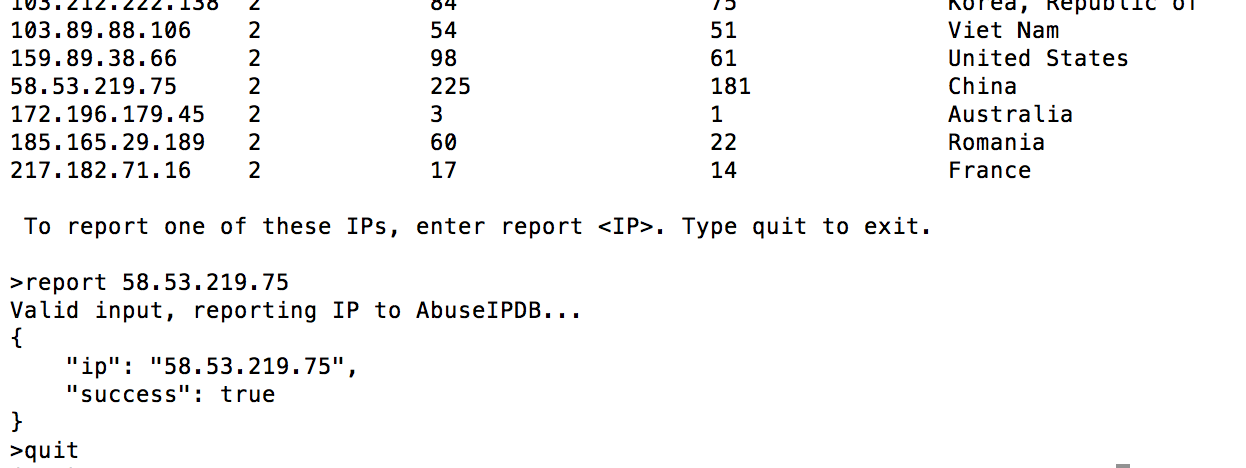
\includegraphics{./figures/561-irpSSHa-prompt.png}}
\caption{\small{Example command prompt interaction}}
\label{fig:prompt}
\end{figure}

\begin{figure}[H]
%\resizebox{\textwidth}{!}
{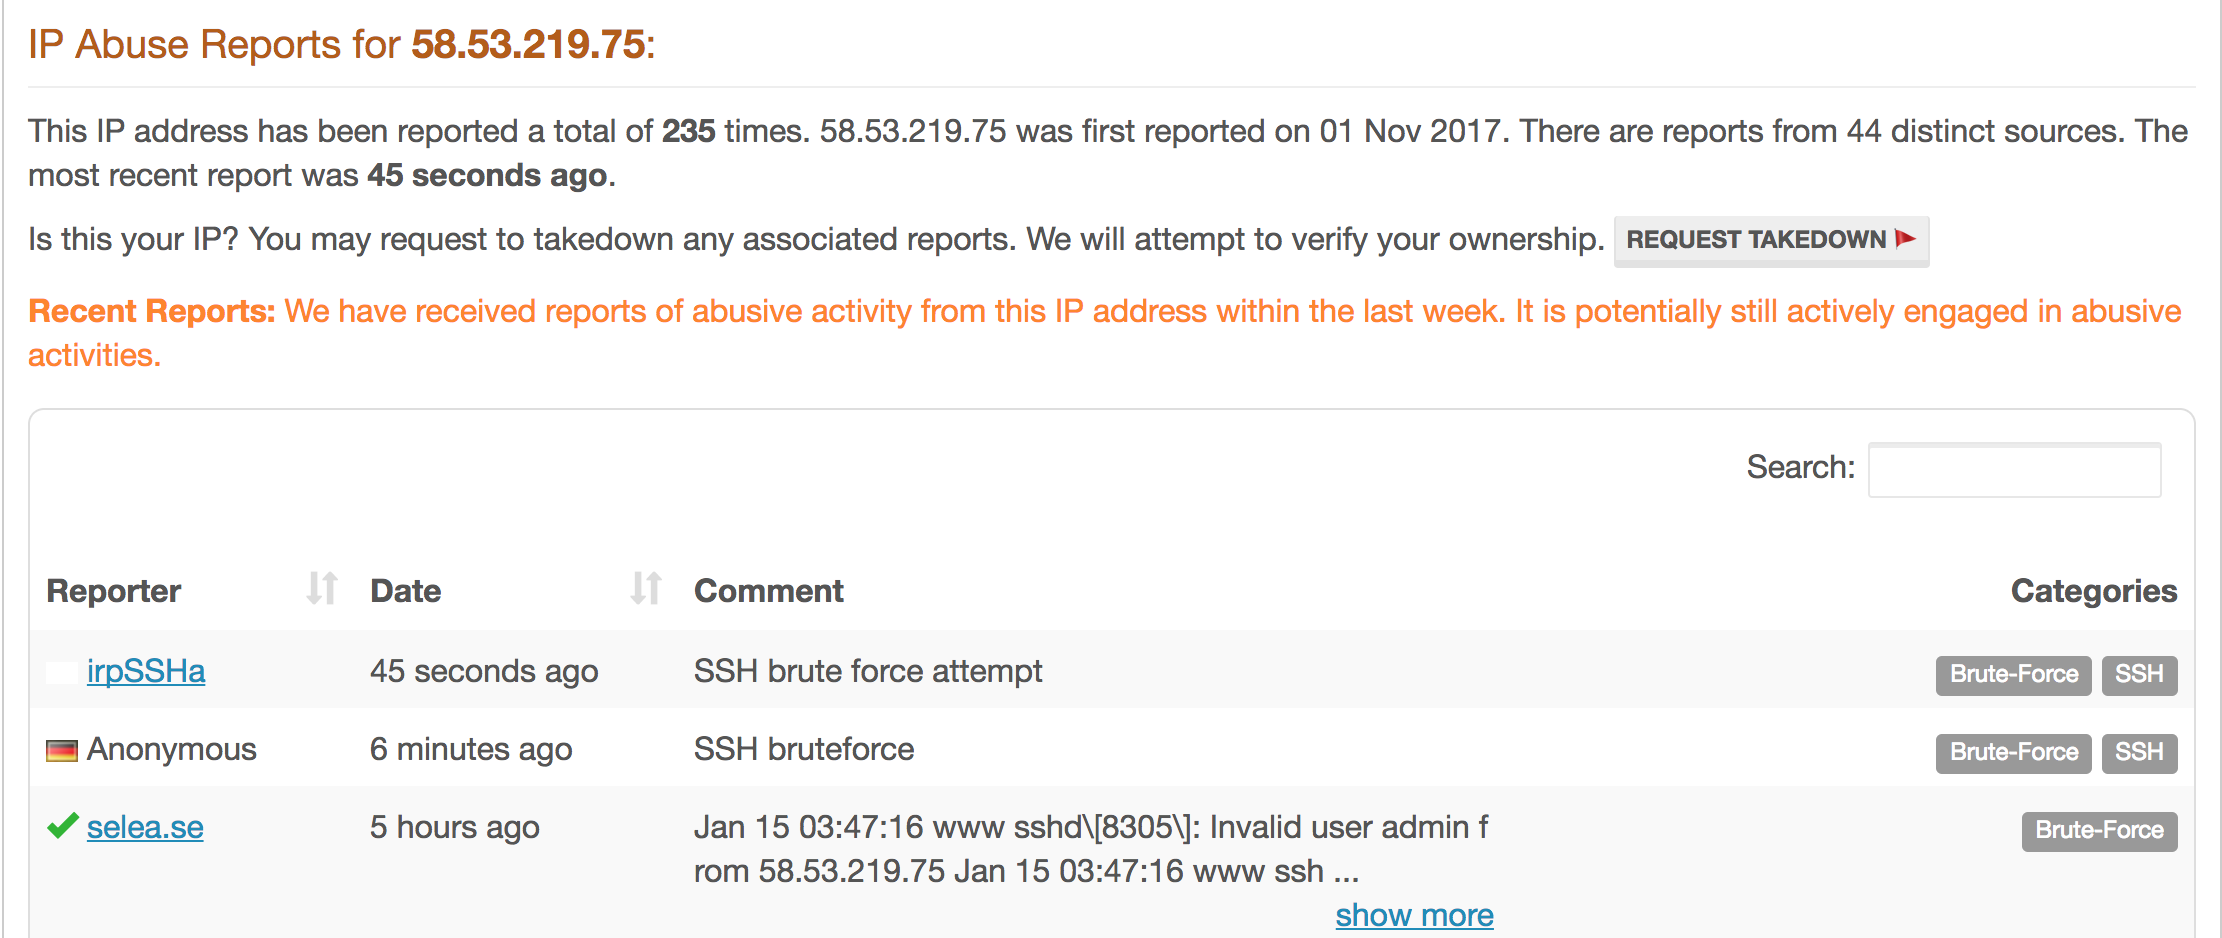
\includegraphics[width=3in]{./figures/561-AbuseIPDB-report.png}}
%{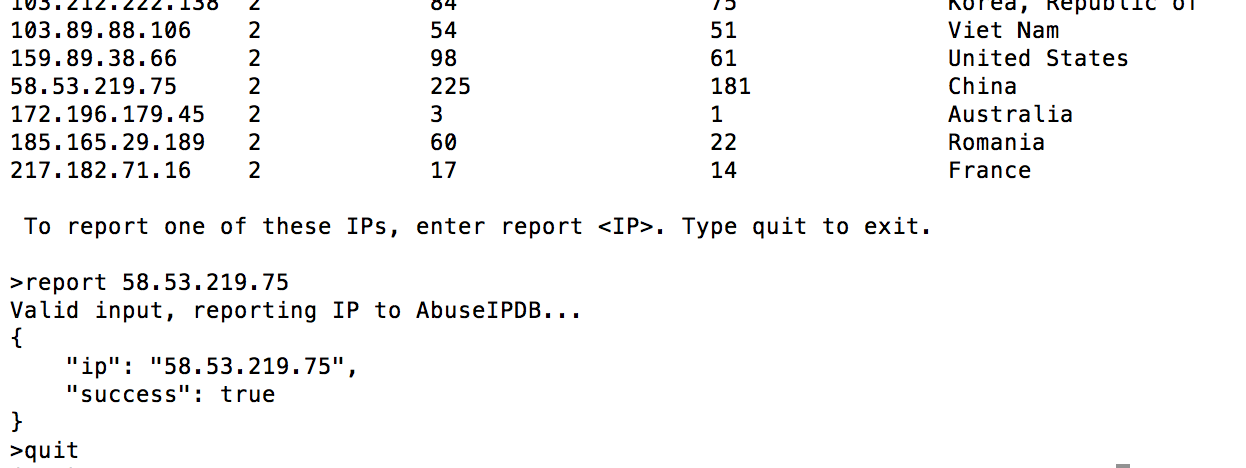
\includegraphics{./figures/561-irpSSHa-prompt.png}}
\caption{\small{Auto-generated report from irpSSHa on AbuseIPDB site}}
\label{fig:report}
\end{figure}

\subsection{Source Code}

The irpSSHa source code is available on GitHub:  \href{https://github.com/jlouthan/irpSSHa}{https://github.com/jlouthan/irpSSHa}.
\label{sec:design}




